% Thank You!
\graphicspath{{Figures/Thank.You/}}

\setbeamercolor{background canvas}{bg=mDarkTeal}
\begin{frame}{}
    \label{Section: Thank You}
    \centering
    \vfill\vspace{1em}\usebeamerfont{section title}\textcolor{white}{\scshape Thank You!}\vfill
\end{frame}

\setbeamercolor{background canvas}{bg=white}

\begin{frame}{Contact Us}
    \label{Thank You: Contact Us}
    Zhang Qi\\
    \href{mailto:qiqi@hust.edu.cn}{\textcolor{blue}{\tt \small qiqi@hust.edu.cn}}\\[10pt]

    Zhou Chunjie\\
    \href{mailto:cjiezhou@hust.edu.cn}{\textcolor{blue}{\tt \small cjiezhou@hust.edu.cn}}\\[10pt]

    Yang Shuanghua\\
    \href{mailto:S.H.Yang@lboro.ac.uk}{\textcolor{blue}{\tt \small S.H.Yang@lboro.ac.uk}}\\[20pt]

%    \pause
%
%    You can obtain this slide from my Github:\\
%    \href{https://github.com/zqmillet/Presentation.for.Loughborough.University}{\tt \small \textcolor{blue}{zqmillet@github.com:Presentation.for.Loughborough.University}}\\[10pt]
%
%    \pause
%    And I have pushed the code of the simulation to my Github, too.\\
%    \href{https://github.com/zqmillet/Multi-level.Bayesian.Network}{\tt \small \textcolor{blue}{zqmillet@github.com:Multi-level.Bayesian.Network}}\\[15pt]
\end{frame}

%\setbeamercolor{background canvas}{bg=mDarkTeal}
\begin{frame}[plain] %{Welcome to HUST}
    \label{Thank You: Welcome to HUST}
    \newlength\FirstHeight
    \newlength\FirstWidth
    \newlength\SecondHeight
    \newlength\SecondWidth
    \newlength\ThirdHeight
    \newlength\ThirdWidth
    \newlength\FourthHeight
    \newlength\FourthWidth
    \newlength\FifthHeight
    \newlength\FifthWidth
    \newlength\SixthHeight
    \newlength\SixthWidth
    \newlength\SeventhHeight
    \newlength\SeventhWidth
    \newlength\EighthHeight
    \newlength\EighthWidth
    \newlength\Interval
    \newlength\Height
    \newlength\Width
    \makebox[\linewidth][c]{%
    \begin{minipage}{\dimexpr\textwidth+5.5em \relax}\centering
    \begin{tikzpicture}[picture/.style = {anchor = north west, inner sep = 0pt},
                        node distance=\Interval and \Interval]
      \setlength\Height{\textheight + 12pt} 
      \setlength\Width{\textwidth - 1pt} 
      \setlength\Interval{2pt} 
      % Image 1
      \setlength\FirstWidth{2.85cm}
      \settoheight\FirstHeight{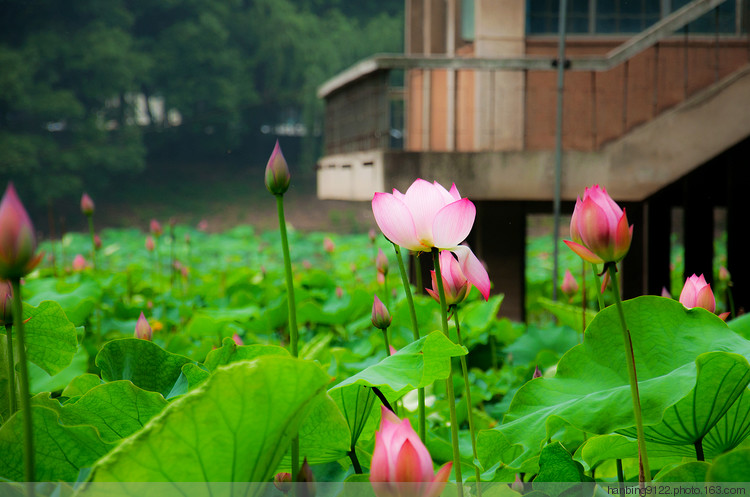
\includegraphics[width=\FirstWidth]{1.jpg}}
      % Image 2
      \setlength\SecondWidth{\FirstWidth}
      \settoheight\SecondHeight{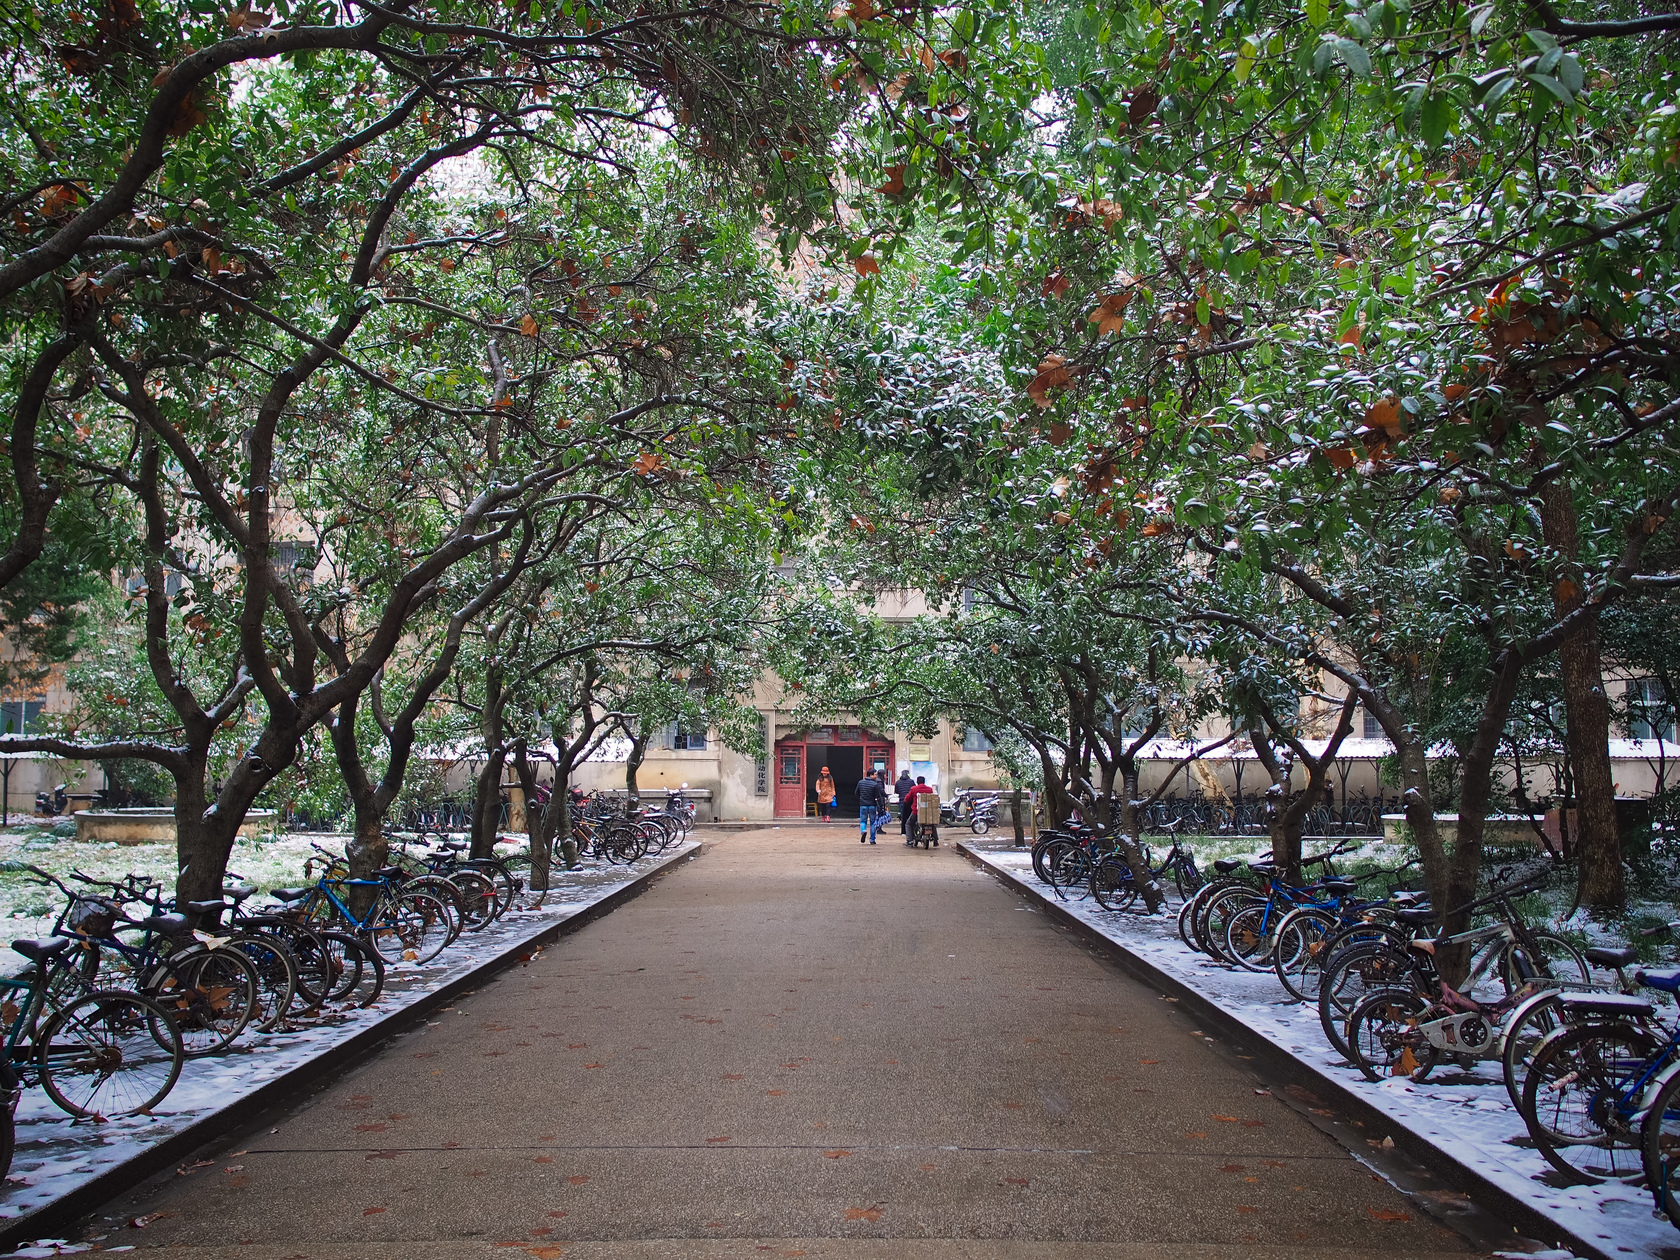
\includegraphics[width=\SecondWidth]{2.jpg}}
      % Image 3
      \setlength\ThirdHeight{\FirstHeight + \SecondHeight + \Interval}
      \settowidth\ThirdWidth{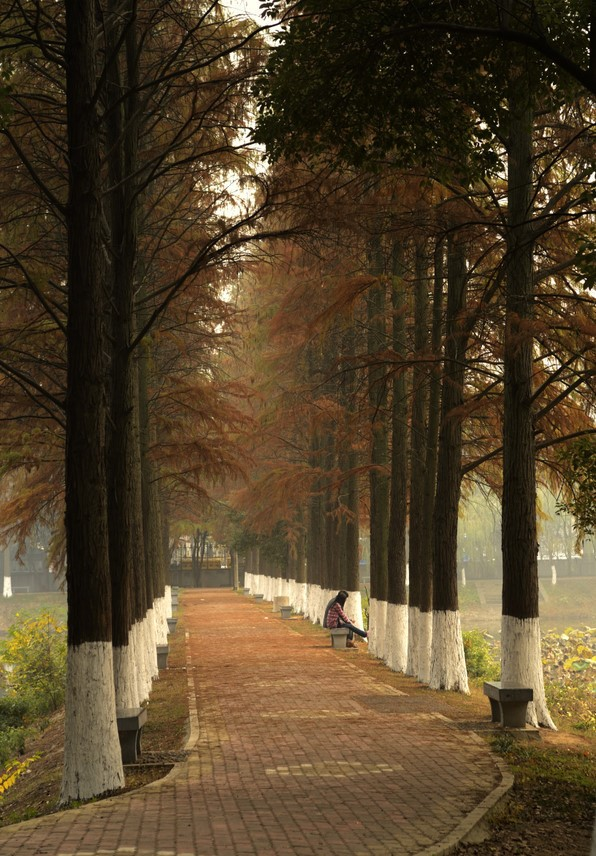
\includegraphics[height=\ThirdHeight]{3.jpg}}
      % Image 7
      \setlength\SeventhHeight{\ThirdHeight}
      \settowidth\SeventhWidth{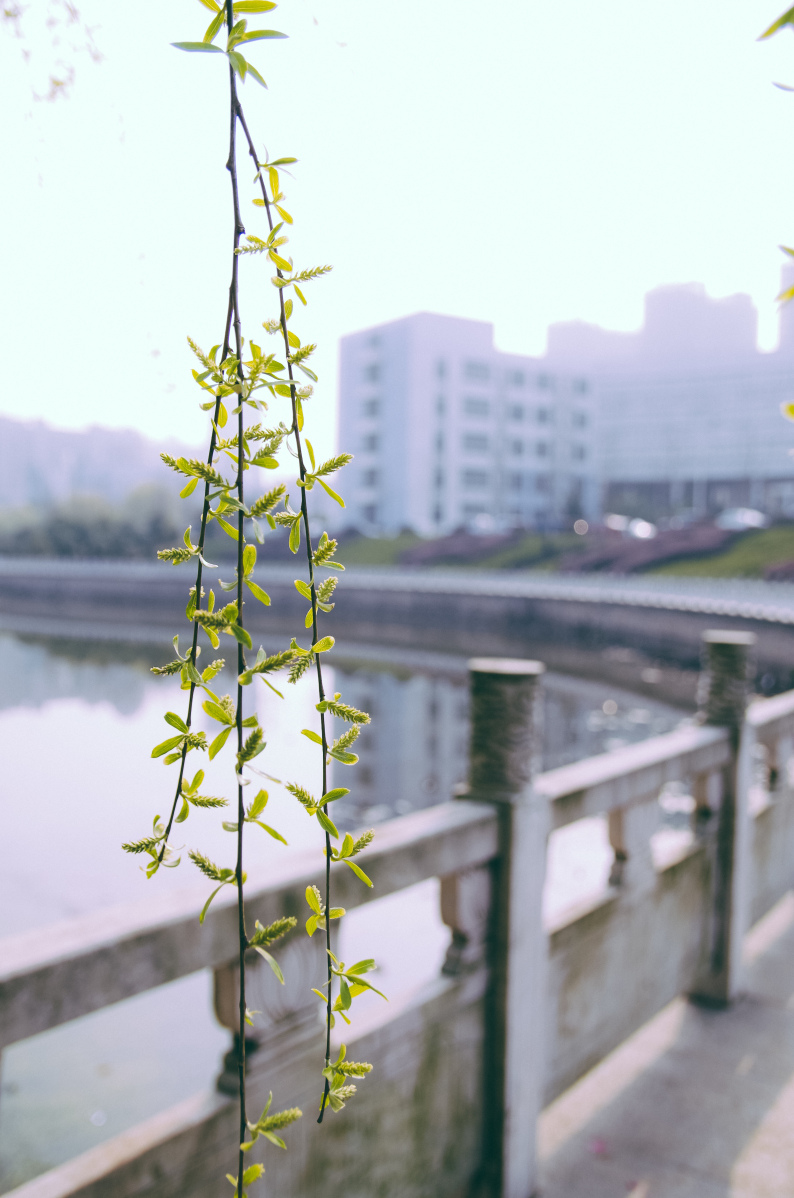
\includegraphics[height=\SeventhHeight]{7.jpg}}
      % Image 6
      \setlength\SixthWidth{\Width - \FirstWidth - \ThirdWidth - \SeventhWidth - 3\Interval}
      \settoheight\SixthHeight{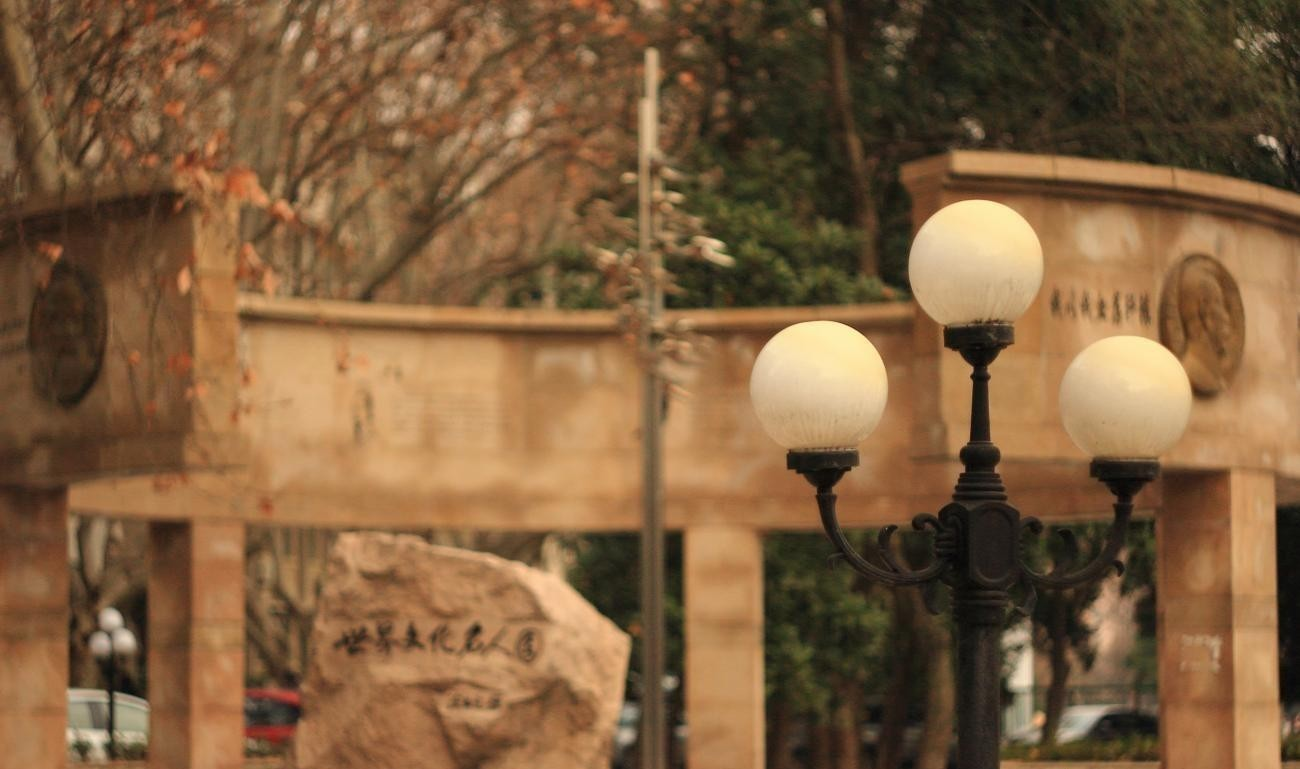
\includegraphics[width=\SixthWidth]{6.jpg}}
      % Image 4
      \setlength\FourthHeight{\ThirdHeight - \Interval - \SixthHeight}
      \settowidth\FourthWidth{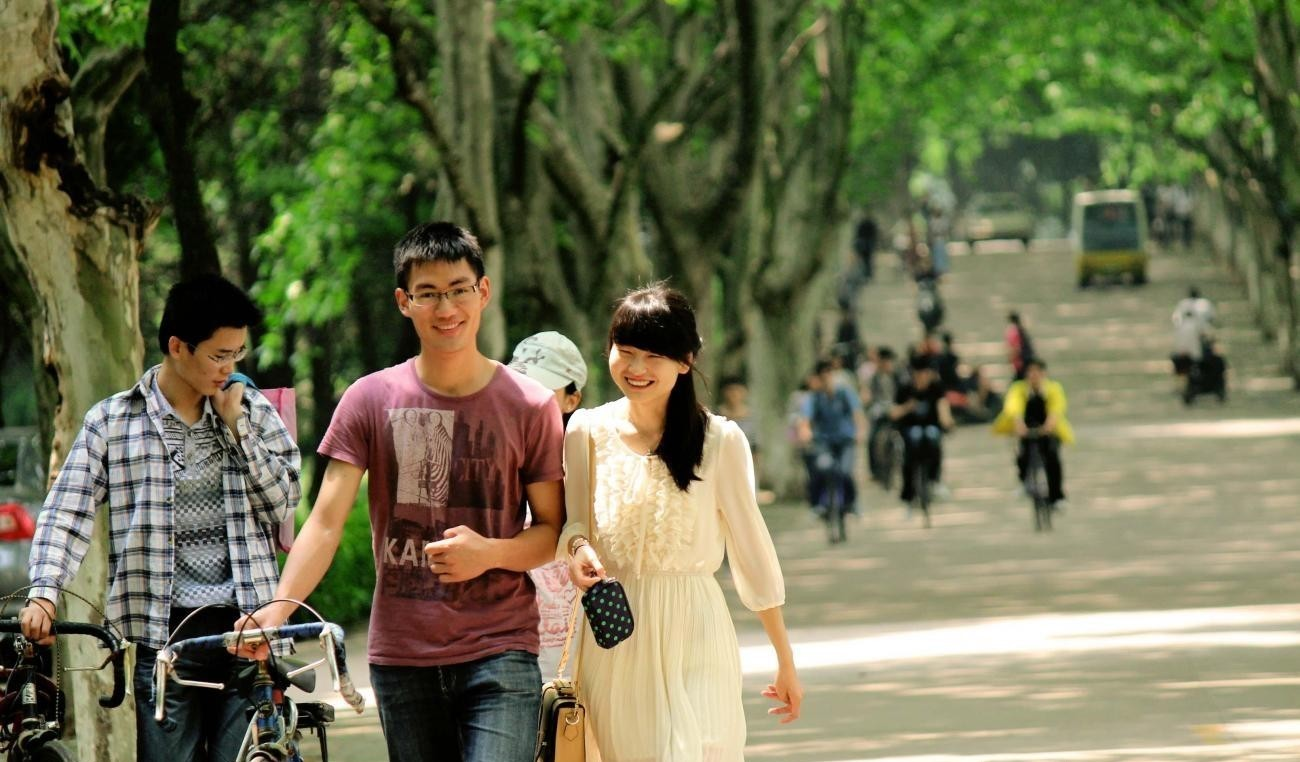
\includegraphics[height=\FourthHeight]{4.jpg}}
      % Image 5
      \setlength\FifthHeight{\FourthHeight}
      \setlength\FifthWidth{\Width - \FirstWidth - \ThirdWidth - \FourthWidth - \SeventhWidth - 4\Interval}
      % Image 8
      \setlength\EighthWidth{\Width}
      \settoheight\EighthHeight{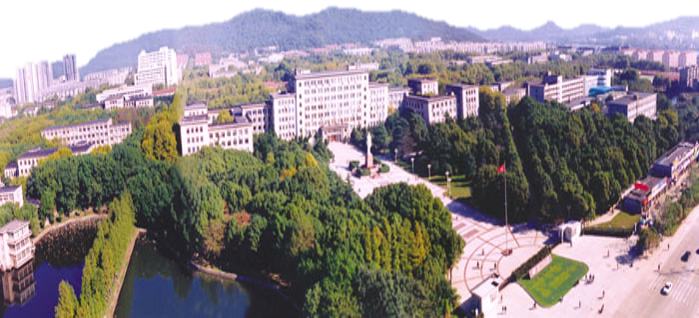
\includegraphics[width=\EighthWidth]{8.png}}


      \node[picture] (1) at (0, \Height)
      {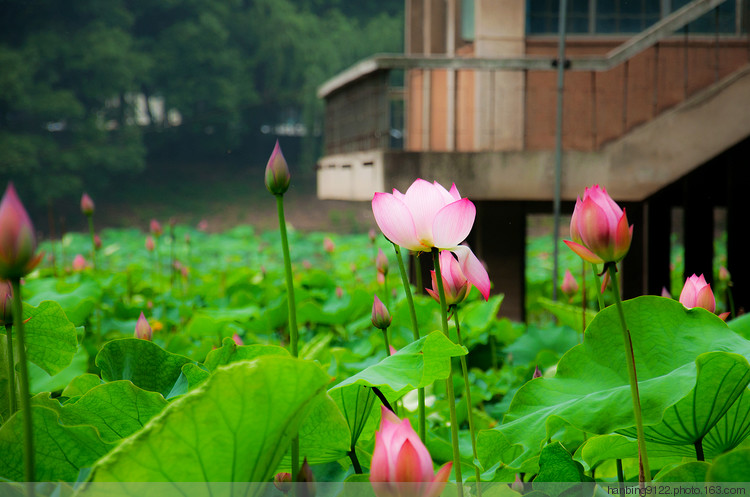
\includegraphics[width=\FirstWidth]{1.jpg}};
      \node[picture] (2) at (0, \Height - \FirstHeight - \Interval)
      {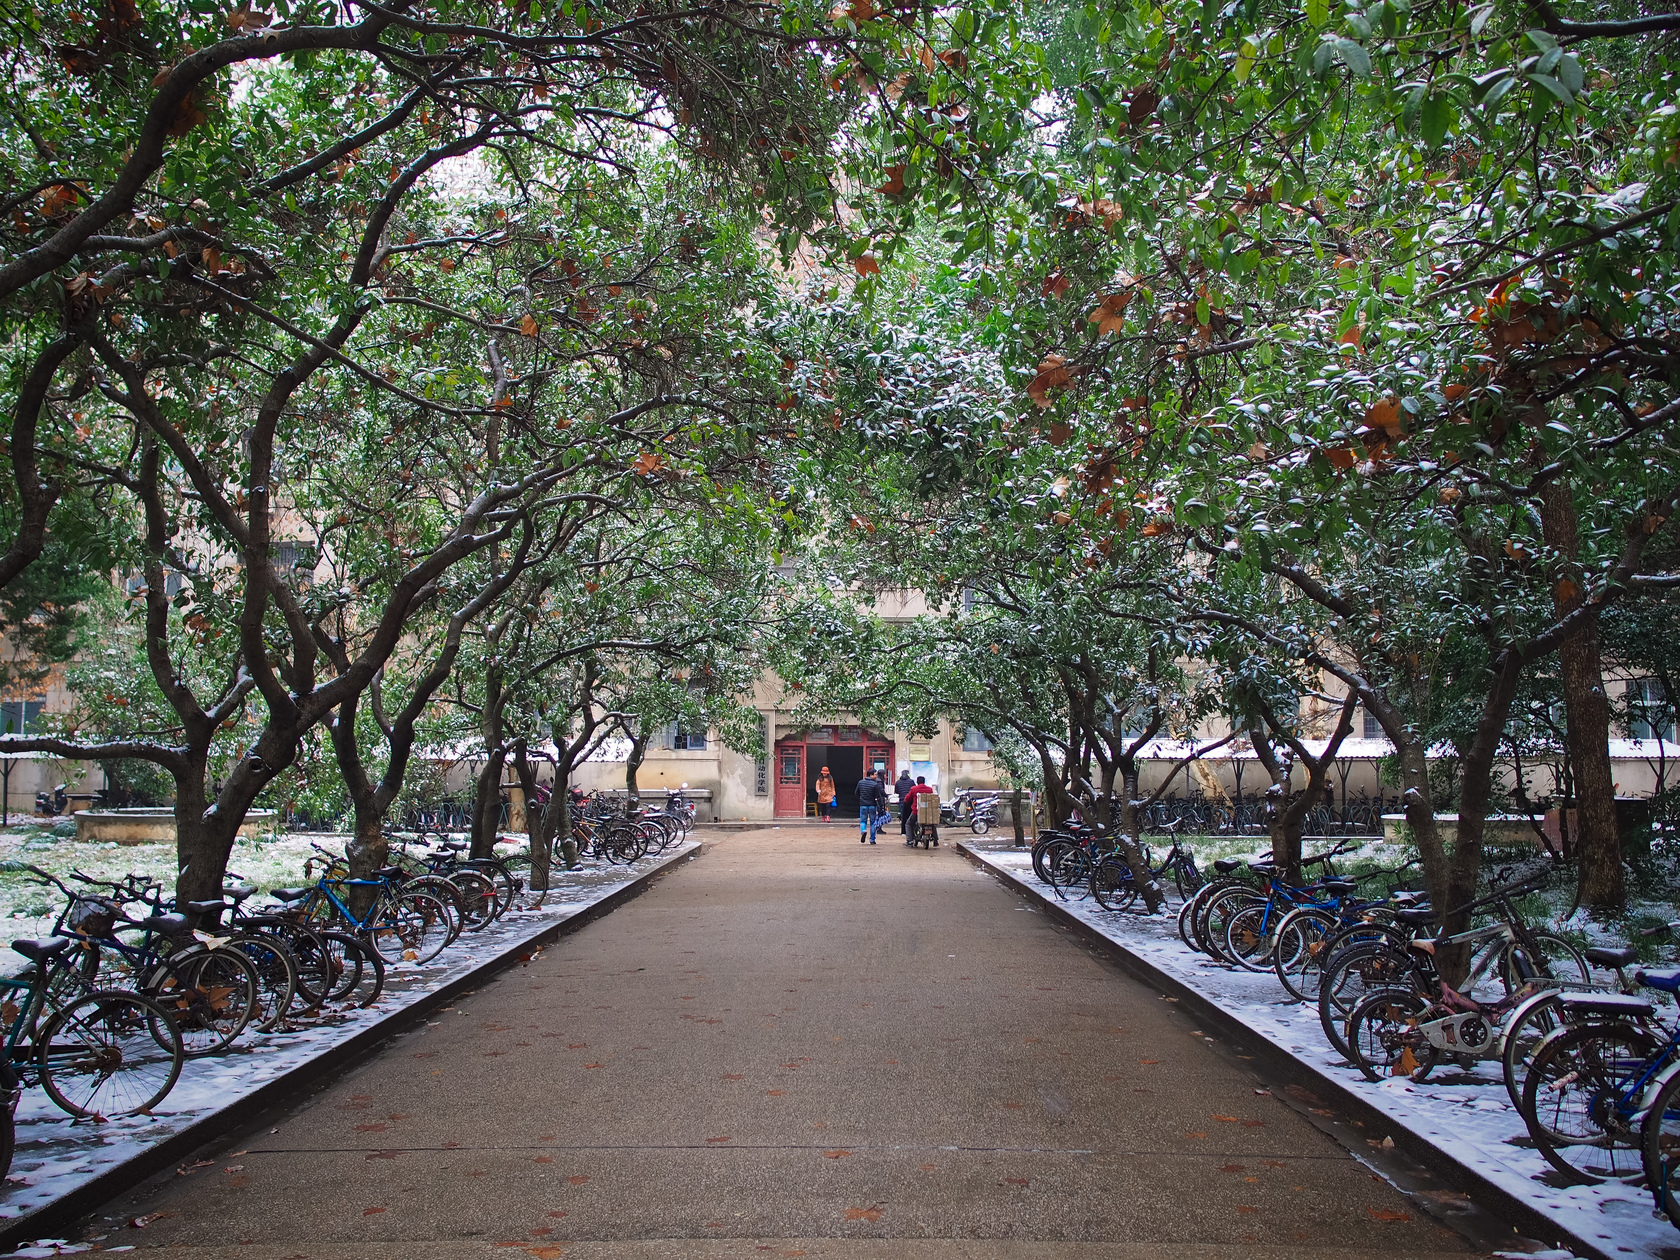
\includegraphics[width=\SecondWidth]{2.jpg}};
      \node[picture] (3) at (\FirstWidth + \Interval, \Height)
      {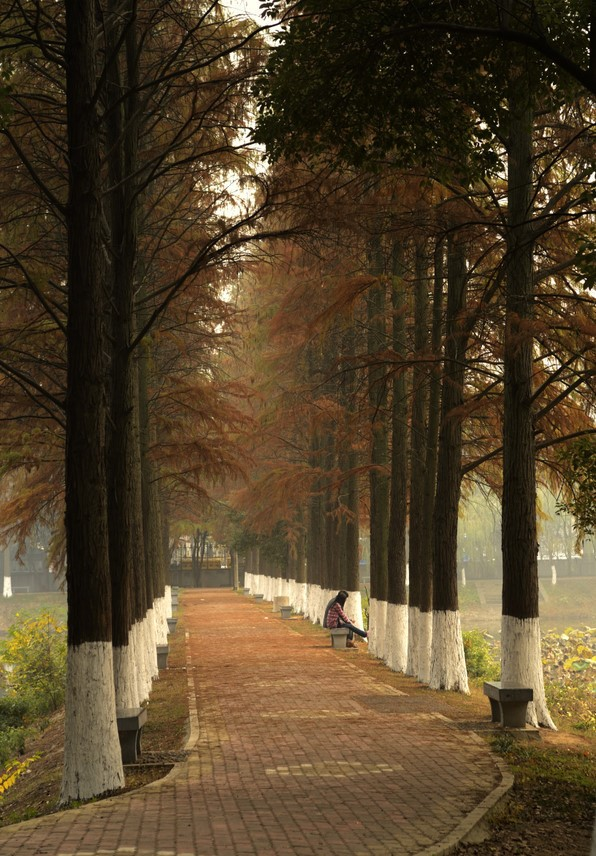
\includegraphics[width=\ThirdWidth]{3.jpg}};
      \node[picture] (4) at (\FirstWidth + \SecondWidth + 2*\Interval, \Height)
      {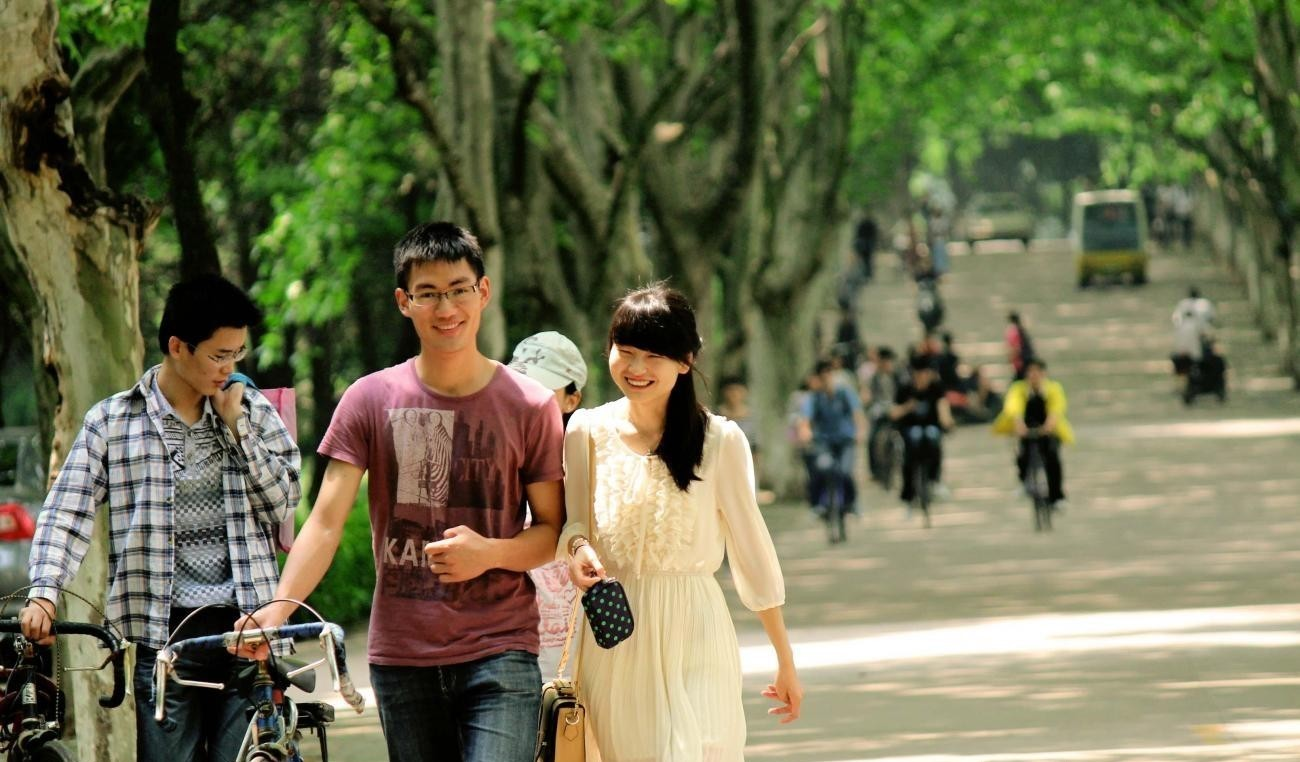
\includegraphics[width=\FourthWidth]{4.jpg}};
      \node[picture] (5) at (\Width - \SeventhWidth - \FifthWidth - \Interval, \Height)
      {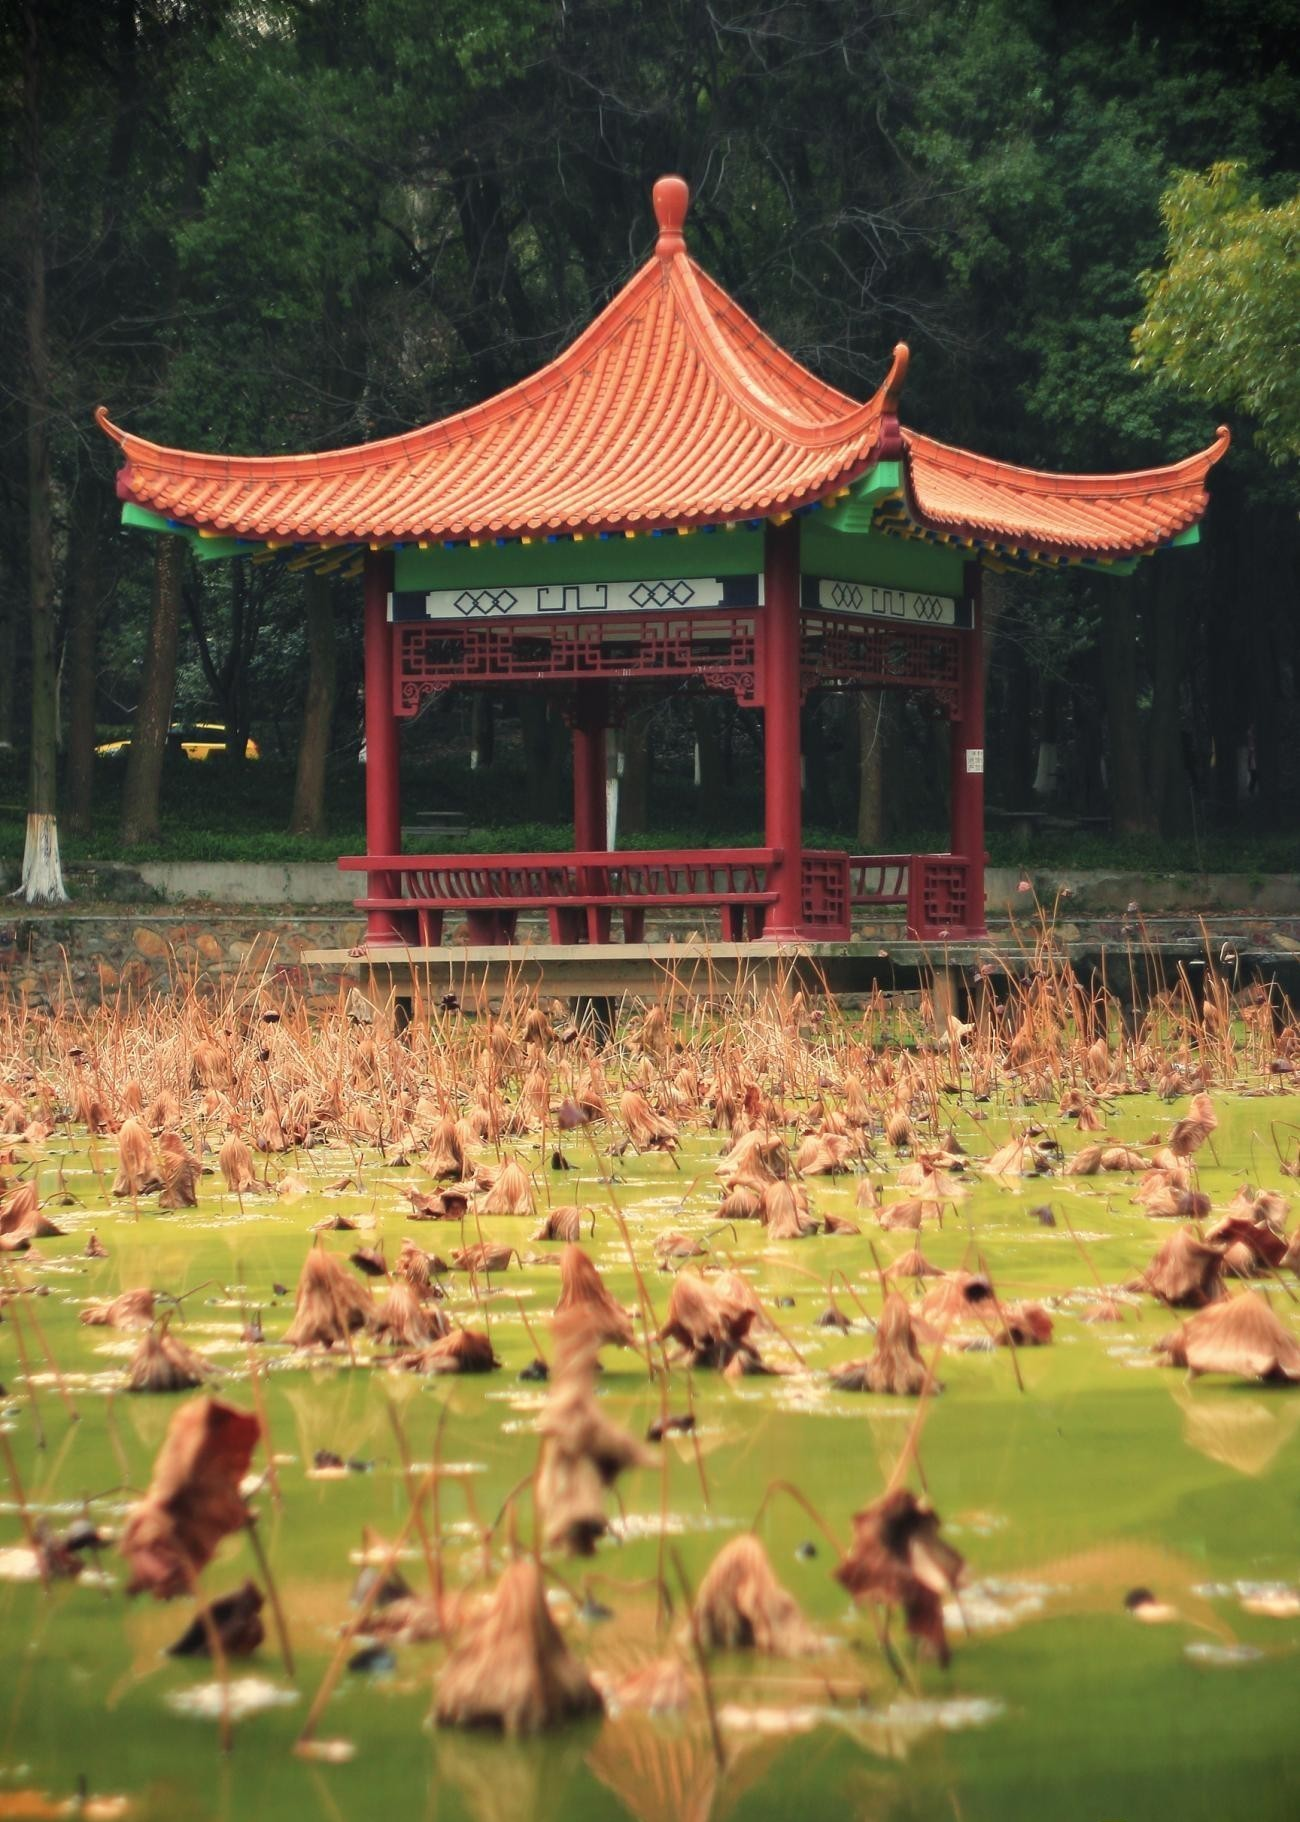
\includegraphics[width=\FifthWidth, height=\FifthHeight]{5.jpg}};
      \node[picture] (6) at (\Width - \SeventhWidth - \SixthWidth - \Interval, \Height - \FourthHeight - \Interval)
      {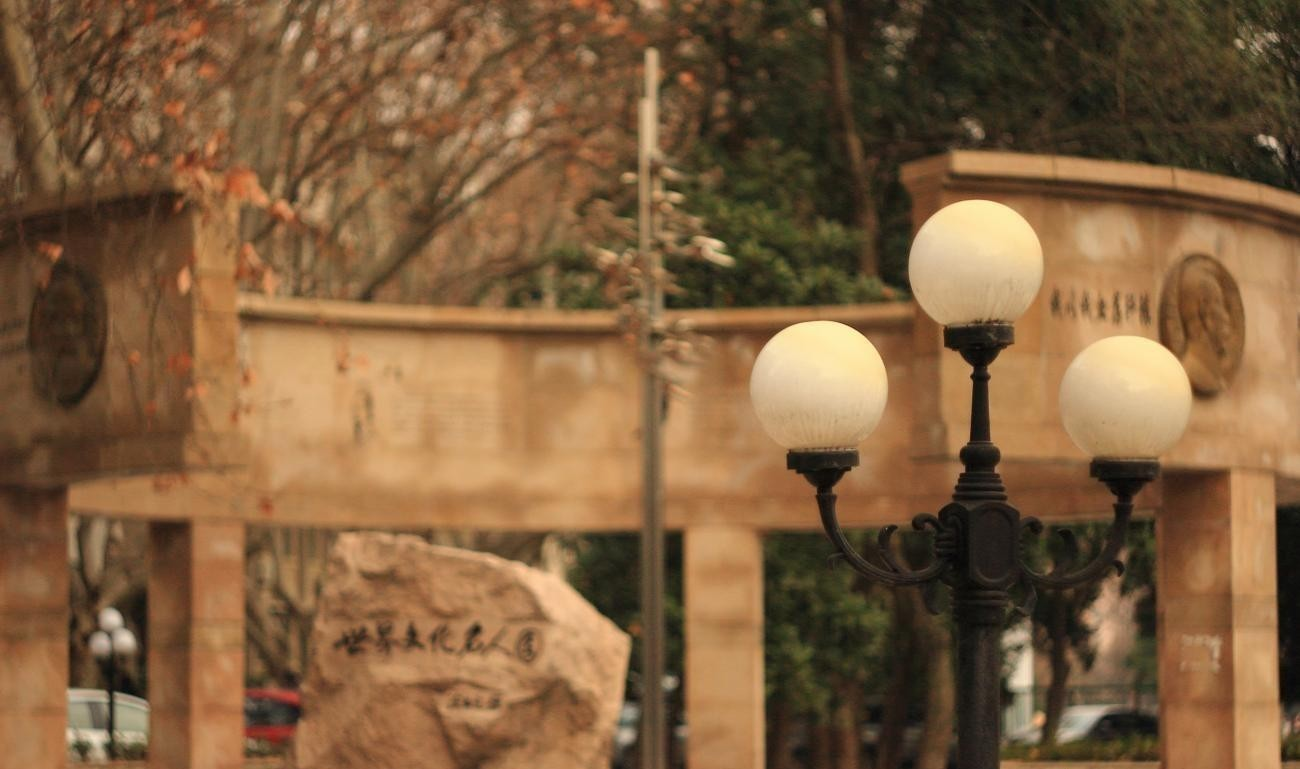
\includegraphics[width=\SixthWidth]{6.jpg}};
      \node[picture] (7) at (\Width - \SeventhWidth, \Height)
      {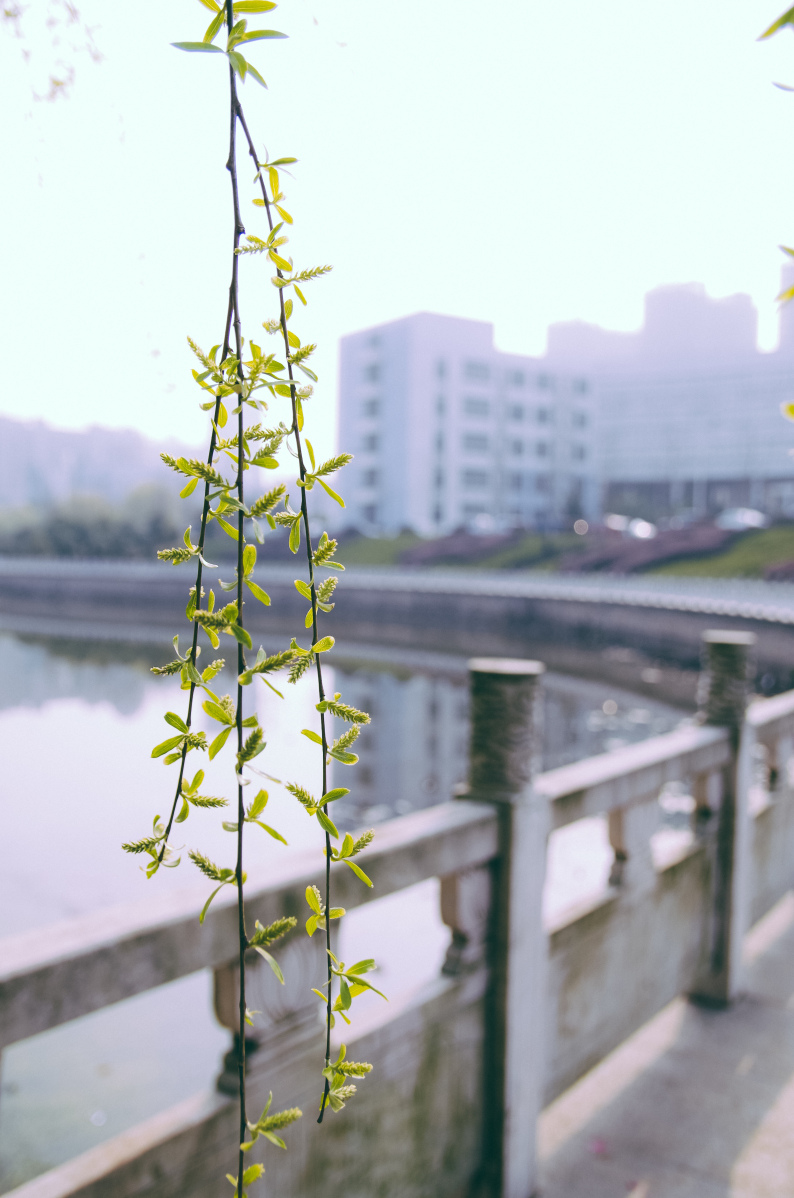
\includegraphics[width=\SeventhWidth]{7.jpg}};      
      
      \node[picture] (8) at (0, \EighthHeight)
      {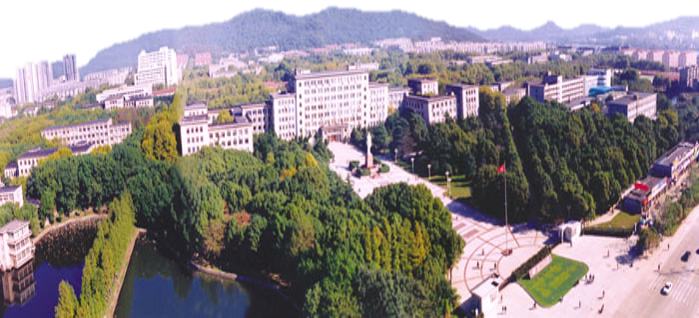
\includegraphics[width=\EighthWidth]{8.png}};
      
      \node at (0.5\Width, 0.5\Height + 0.5\EighthHeight - 0.5\ThirdHeight) {\scalebox{3}{\Black \textcolor{black}{Welcome to HUST!}}};
    \end{tikzpicture}
    \end{minipage}%
    }%

\end{frame}

% Questions
\setbeamercolor{background canvas}{bg=mDarkTeal}
\begin{frame}{}
    \label{Section: Questions}
    \centering
    \vfill\vspace{1em}\usebeamerfont{section title}\textcolor{white}{\scshape Any Questions?}\vfill
\end{frame} 